\documentclass[a4paper]{article}
\usepackage{lscape}
\usepackage[utf8]{inputenc}
\usepackage{tikz}
\usepackage[T1]{fontenc}
\usepackage[polish]{babel}
\usepackage{graphicx}
\usepackage{pdfpages}
\graphicspath{ {./charts/} }
\usepackage{minted}
\usepackage{caption}
\usepackage[a4paper,top=2cm, total={6in, 8in}]{geometry}




\renewcommand{\contentsname}{Spis treści}
\def\checkmark{\tikz\fill[scale=0.4](0,.35) -- (.25,0) -- (1,.7) -- (.25,.15) -- cycle;} 
\title{Sprawozdanie z projektu: Bazy danych 1\\Baza danych pływalni}

\author{Leszek Błażewski, 241264 \\ \\Karol Noga, 241259}

\date{Semestr letni 2018/2019}

\begin{document}
\maketitle
\thispagestyle{empty}
\clearpage
\setcounter{page}{1}
\tableofcontents
\newpage{}

\section{Wstęp teoretyczny}

Poniższy rozdział traktuje o wiedzy nabytej w trakcie wykładów oraz podczas realizacji projektu. Przedstawiono w nim najważniejsze informacje związane z relacyjnym modelem danych oraz teorię pozwalającą lepiej zrozumieć schemat późniejszej implementacji.

\subsection{Podstawy relacyjnych baz danych}

Pierwszym pojęciem, które wymaga definicji w celu zrozumienia działania relacyjnych baz danych jest koncepcja modelu bazodanowego. \textbf{Baza danych} jest uporządkowanym zbiorem logicznie powiązanych ze sobą informacji, której zadaniem jest odwzorowanie fragmentu rzeczywistości w sposób spójny, ułatwiający przechowywanie oraz przeszukiwanie danych. Dane przechowany w bazie mogą stanowić byty abstrakcyjne, lecz muszą być zgodne z rzeczywistością oraz muszą być trwałe.

Model relacyjny po raz pierwszy zdefiniowany został przez Edgara Franka Codda, w \textit{1970} roku w pracy pod tytułem \textit{A Relational Model of Data for Large Shared Data Banks.}. Praca ta stanowi fundament modelu relacyjnego, definiując jego główne założenia oraz zawiera formalne operatory przeszukiwań danych.

\textbf{Model relacyjny} jest sposobem prezentacji oraz manipulacji danych, dotyczącym struktury danych jako relacji, integralności danych oraz operacji na danych poprzez selekcję, projekcję oraz operacje na zbiorach. W modelu relacyjnym dane reprezentowane są w postaci tabel (relacji) na których dokonywać można działań przy pomocy podstawowych operatorów algebry relacyjnej. Każda tabela posiada własny zestaw atrybutów (kolumn), które przyjmują wartości z określonej dziedziny. Relacja odwzorowująca związki pomiędzy tabelami w bazi definiowana jest w poniższy sposób.

Relacja $r(R)$ o schemacie $R(A_1,A_2,...,A_n)$ na zbiorze dziedzin $\{D_1,D_2,...,D_n\}$jest zbiorem krotek $r=\{t_1,t_2,...,t_m\}$ postaci $t=< v_1,v_2,...,v_n>$, będących uporządkowaną listą, gdzie $v_i$, dla $0 < i \leq n $ należy do zbioru $D_i\cup\{NULL\},n$ jest stopniem relacji $R$, natomiast $m$ stanowi jej liczebność.

W celu zagwarantowania integralności danych przechowywanych w bazie zdefiniowano szereg reguł, które stanowią podstawę dla systemu zarządzania bazą danych do nadzoru poprawności wprowadzanych danych. Ograniczenia te mogą dotyczyć pojedynczego atrybutu bądź, całej relacji. Wyróżniamy poniższe ograniczenia:
\begin{itemize}
    \item klucze główne \textit{(PRIMARY KEY)}
    \item klucze obce \textit{(FOREIGN KEY)}
    \item unikalność \textit{(UNIQUE)}
    \item zawężanie dziedziny \textit{(CHECK})
    \item wartość nie pusta \textit{(NOT NULL)}
\end{itemize}

Klucze główne pozwalają jasno identyfikować daną relację, natomiast klucze obce stanowią referencję do krotki docelowej zawierającej wartość odpowiadającego mu klucza głównego. Restrykcja \textit{UNIQUE}, ogranicza wartości danego atrybuty lub kombinacji atrybutów jedynie do unikalnych w stosunku do innych znajdujących się w bazie. Ograniczenie \textit{CHECK}, pozwala na nałożenie warunku na daną kolumnę, dzięki czemu możemy ograniczyć dziedzinę danych atrybutów, tym samym gwarantując integralność bazy. Ostatnia z restrykcji blokuje możliwość wprowadzenia wartości \textit{NULL}, dla danej kolumny.

\newpage

W celu utworzenia poprawnego schematu bazy danych, pierwszy etap projektowania obejmuje modelowanie pojęciowe oparte o encje. \textbf{Model pojęciowy} jest abstrakcyjnym opisem rzeczywistych obiektów. Pozwala on określić zależności występujące pomiędzy konkretnymi encjami oraz obrazuje w prosty sposób schemat przyszłej bazy. Model pojęciowy najczęściej reprezentowany jest w postaci diagramu związków encji \textit{ERD} lub diagramu \textit{UML}. Modelowanie pojęciowe opiera się na poniższych założeniach:
\begin{itemize}
    \item modelowany świat składa się z encji
    \item encje mogą być grupowane w typy
    \item każda encja posiada własność, która ją identyfikuje
    \item encje są ze są powiązane
\end{itemize}

Poniżej zamieszczono sposób interpretacji powyższych zasad modelowania na przykładzie jednej z encji w modelowanej bazie danych.

\begin{table}[htbp]
\centering
\begin{tabular}{|c|c|c|}
\hline
\textbf{pojęcie} & \textbf{znaczenie} & \textbf{przykład}                             \\ \hline
encja            & dany obiekt        & basen, ratownik                               \\ \hline
własność         & opisuje encję      & ilość miejsc, zarobki                         \\ \hline
związek          & łączy encje        & praca(basen - ratownik)                       \\ \hline
podtyp           & podtyp encji       & młodszy ratownik jest typem niższym ratownika \\ \hline
\end{tabular}
\caption{Przykład opisu encji}
\end{table}

\textbf{Encja} reprezentuje  zbiór  obiektów  w  modelowanym  fragmencie  rzeczywistości, które posiadają te same cechy i są na tyle istotne, by trwale przechowywać o nich informacje. Każda encja posiada zbiór cech, który obejmuje jej własności oraz unikalną nazwę i identyfikator. Istotne jest też założenie, traktujące o możliwości reprezentacji dowolnego obiektu wyłącznie przez jedną encję. Encje mogą reprezentować:
\begin{itemize}
    \item obiekty materialne - kasjerka, basen, klient
    \item obiekty niematerialne - harmonogram pracy
    \item zdarzenia - rezerwacja
    \item fakty - stan magazynowy
\end{itemize}

Wyróżniamy również encje słabe, których istnienie zależne jest od innej encji występującej w bazie danych. Przykładem encji słabej w implementowanej bazie danych może być rozpiska zmian pracownika, która istnieje jedynie gdy dana encja pracownika znajduje się w bazie, a w momencie zwolnienia pracownika jego zmiany również są usuwane.

Ważnym etapem podczas definiowania danych encji jest określenie ich własność, które wymaga rozpatrzenia kilku warunków. \textbf{Definicja własności} dla danej encji obejmuje:
\begin{enumerate}
    \item określenie nazwy encji
    \item określenie dziedziny - typ danych, ich rozmiar oraz zakres dozwolonych wartości
    \item dopuszczenie/niedopuszczenie wartości \textit{NULL}
    \item opcjonalne zdefiniowanie warunku unikalności
\end{enumerate}

Ostatnim etapem projektowania bazy relacyjnej jest określenie związków występujących pomiędzy danymi encjami. \textbf{Związki} określają zbiór asocjacji pomiędzy instancjami danych encji i stanowią odwzorowanie pomiędzy obiektami świata rzeczywistego. Liczba encji wchodzących w dany związek określa jego stopniem. Wyróżniamy następujące typy związków:
\begin{itemize}
    \item unarne, binarne, ternarne
    \item obligatoryjne lub opcjonalne
    \item jeden do jednego, jeden do wielu, wiele do wielu
\end{itemize}

\textbf{Związki unarne} wiążą instancję danej encji z instancją takiego samego typu. W wielu przypadkach związek unarny reprezentuje rekurencyjne powiązanie hierarchiczne. Jako przykład posłużyć możemy się relacją pracownik - przełożony w projektowanej bazie danych. Każdy pracownik posiada kolumnę \textit{SUPERVISOR}, która stanowi klucz obcy przechowujący \textit{ID} pracownika, który jest kierownikiem danej osoby.

\textbf{Związki binarne} są najczęstszym typem związków występujących w relacyjnych bazach danych. Wiążą one instancje dwóch różnych encji. Ponieważ nasza baza opiera się w głównej mierze na związkach ternarnych, nie wykorzystaliśmy łączeń binarnych. Natomiast przykładem takiego wiązania może być połączenie mieszkańca z jego miejscem zamieszkania.

\textbf{Związki ternarne} stanowią połączanie trzech osobnych encji. Przykładem związku ternarnego w implementowanej bazie jest relacja pomiędzy encjami \textit{POOL} a  \textit{STAFF}, która łączy danego pracownika i jego czas pracy z basenem do którego jest przydzielony, przechowując dane w encji \textit{SCHEDULES}.

Dla każdego typu związku wyróżniamy również typy asocjacyjne, które omówione zostaną dokładniej w rozdziale dotyczącym modelu danych \textbf{ERD}.

\newpage

\subsection{Normalizacja} \label{Redundancja}

\subsubsection{Normalizacja bazy danych a redundancja}

Proces normalizacji bazy danych polega na doprowadzaniu bazy do postaci w której w bazie nie występuje redundancja. Redundancja jest zjawiskiem na ogół niepożądanym, lecz w specyficznych przypadkach jest konieczna w celu zapewnienia jakości danych usług (np. redundancja serwerów). Rozważając redundancję ze względu na dane występujące w bazie zauważyć możemy, że zjawisko to nie przynosi żadnych korzyści a jedynie przechowuje dane, które składowane są już w bazie tym samym zajmując miejsce, które wykorzystane mogłoby być na nowe informacje. Do redundancji dochodzić może gdy relacje pomiędzy obiektami nie zostały dokładnie przemyślane.

\subsubsection{Proces normalizacji}

Podczas pierwszej implementacji, nie zwróciliśmy uwagi na relacje zachodzące pomiędzy encją pracownika pływalni a jego czasem oraz dniami pracy. Pierwszym pomysłem było przechowywanie wszystkich danych dotyczących danego pracownika (włącznie z czasem pracy, dniami tygodnia gdy dana osoba pracuje oraz basenem do którego jest przydzielona) w tabeli $STAFF$. Takie rozwiązanie powodowało znaczne zwiększenie rozmiaru rekordów, co niekorzystnie wpłynęłoby na czas przeszukiwania danej tabeli. Problematyczne byłoby również przeszukiwanie tabeli w celu znalezienia pracowników pracujących w danych dniach, ponieważ każdy z rekordów odpowiadających danemu pracownikowi przechowywałby listę dni tygodnia przetrzymywaną w jednej kolumnie $WORKINGDAYS$, co kłóci się z pierwszą postacią normalną $(1NF)$.

Rozwiązaniem problemu jest wprowadzenie osobnej tabeli $SCHEDULES$, która abstrahuje dane dotyczące czasu pracy oraz dni tygodnia od reszty informacji dotyczących pracownika. Tabela $SCHEDULES$ przechowuje klucz obcy do pracownika oraz do basenu, dzięki czemu znacznie redukujemy liczbę kolumn w tabeli i korzystamy z relacji klucz obcy -> główny. Rozwiązanie to też w prosty sposób pozwoliło uniknąć problemu przetrzymywania listy dni w jednej kolumnie, dzięki czemu pierwsza zasada postaci normalnej zostaje zachowana.

\section{Część praktyczna}

Poniższa część dokumentu stanowi pełną specyfikację realizowanego projektu wraz z wszystkimi wymaganiami oraz zastosowanymi technologiami.

\subsection{Poruszany problem}

Głównym celem projektu było zaprojektowanie bazy danych, która pozwoli na wsparcie systemu zarządzania pływalnią. Projektowana baza miała ułatwić przepływ oraz składowanie informacji podczas wykonywania podstawowych operacji związanych z procesami zachodzącymi w trakcie działania pływalni.

Odpowiednie składowanie danych oraz relacje zachodzące między poszczególnymi encjami stanowią kluczową kwestię od której w głównej mierze zależy szybkość wykonywania operacji związanych z administracją pływalni. Poprawnie zamodelowana baza danych pozwoli na przyśpieszenie działań mających na celu znalezienie informacji, ułatwi ich składowanie oraz pozwoli na łatwą aktualizację danych wartości.

Do głównych danych, które przetwarzane będą przez system zarządzania pływalnią, należą informacje o klientach oraz ich rezerwacjach, dane pracowników wraz z rozpiską ich godzin pracy oraz informacje dotyczące basenów. Wszystkie wymienione informacje są ze sobą ściśle powiązane w związku z czym należało dokładnie przemyśleć sposób zamodelowania wiązań pomiędzy encjami, tak aby możliwie najlepiej oddawały rzeczywisty stan pływalni oraz spełniały zasady normalności i nie naruszały integralności bazy.

Projekt stworzonej bazy pozwala na zarządzanie rezerwacjami dokonywanymi przez klientów, informacjami dotyczącymi basenów, które wchodzą w skład pływalni oraz danymi pracowników i ich czasem pracy. Największą trudność podczas projektowania, stanowiło poprawne zamodelowanie rozkładu zmian pracowników, ponieważ wymagało ono przechowywania informacji o każdej zmianie. Idealnym rozwiązaniem okazała się tabela asocjacyjna, która w rzeczywistości stanowić mogłaby plan zmian w której dany pracownik zapisuje swój numer identyfikacyjny, czas oraz datę zmiany wraz z numerem identyfikującym basen na którym pracuje.

Stworzony model bazy relacyjnej służyć może do obsługi małego ośrodka. Natomiast w przypadku większych obiektów okazać się może, że zaproponowany schemat nie będzie wystarczający. Podczas projektowania i późniejszej implementacji staraliśmy się aby nasz projekt był w pełni skalowany i prosty w rozbudowie, dzięki czemu w razie potrzeby istnieje możliwość rozwijania schematu bazy bez potrzeby naruszenia obecnych wiązań pomiędzy encjami.

\subsection{Wymagania systemu} \label{Wymagania}

Ponieważ jest to projekt akademicki, część wymagań została spłaszczona, natomiast w rzeczywistych warunkach rozważyć należałoby dodatkowe encje, które dostarczałyby dalszych informacji o stanie pływalni. Zaprojektowana baza stanowi jedynie podstawę do zbudowania systemu pozwalającego na kompleksową obsługę całej instytucji. Niemniej jednak zbudowany model jest łatwy w implementacji oraz pozwala na swobodną rozbudowę i dokładanie kolejnych zależności czy nowych encji.

Głównym wymaganiem budowanego modelu bazy danych było dostarczenie rozwiązania, które pozwoli efektywnie rozwiązać poniższe kwestie:
\begin{itemize}
    \item Przechowywanie danych klientów.
    \item Przetrzymywanie danych związanych z obecnym stanem basenów.
    \item Zapis rezerwacji poszczególnych klientów.
    \item Automatyczna archiwizacja rezerwacji.
    \item Zarządzanie danymi pracowników.
    \item Możliwość łatwego sprawdzenia oraz aktualizacji czasu pracy danych osób.
\end{itemize}

\textbf{Dane klientów} składać się miały z: imienia, nazwiska, numeru pesel, opcjonalnego numeru telefonu oraz wieku. Uważać można, że pole wieku jest nadmiarowe i stanowi redundancję w stosunku do numeru pesel, jednak postanowiliśmy zawrzeć to pole, ponieważ schemat obliczenia wieku na podstawie numeru pesel jest czasochłonny i znacznie komplikuje procesy bazujące na wieku klienta.

\textbf{Informacje związane z basenami} składały się jedynie z numeru identyfikującego dany basen, ilości dostępnych miejsc oraz ceny za miejsce. Jednym z wymagań projektowych było odwzorowanie w bazie sytuacji w której dane baseny dostępne są jedynie dla osób, które osiągnęły wymagany poziom umiejętności. Dodatkowo należało uwzględnić możliwość basenów dla których poziom trudności nie był zdefiniowany tzn. były one dostępne dla każdego klienta niezależnie od jego poziomu umiejętności. Następnie należało zapewnić pełną zgodność danych dotyczących ilości rezerwacji na dany basen, uwzględniając liczbę dostępnych miejsc.

\clearpage

\textbf{Rezerwacje klientów} zawierane miały być przez danego klienta o zadanym numerze identyfikacyjnym, na dany basen, do którego miał dostęp, to znaczy jego poziom umiejętności był równy lub przekraczał wymagany poziom na basenie. Rezerwacje miały być również dokonywane na daną datę i czas. Cena rezerwacji zależna miała być od ceny miejsca na danym basenie. Dodatkowym wymaganiem dotyczącym rezerwacji było automatycznie zmniejszenie ceny o połowę lub 25\% odpowiednio, gdy dana rezerwacja zawierana była przez osobę niepełnoletnią lub klienta, którego wiek równy był lub przekraczał 75 lat. Kolejnym wymaganiem było zdefiniowanie automatycznego procesu archiwizacji rezerwacji danych klientów oraz odpowiednia aktualizacja ilości dostępnych miejsc na danym basenie w momencie rezerwacji lub po jej usunięciu. Całość odbywać się miała cyklicznie co 30 minut, usuwając rezerwacje, których godzina zakończenia starsza jest od obecnego czasu, przywracając odpowiednią ilość miejsc na basenach oraz archiwizując usuwane rekordy.

\textbf{Dane pracowników} zawierać miały unikalny identyfikator pracownika, imię, nazwisko, zarobki, wykonywany zawód oraz opcjonalne pole, identyfikujące przełożonego danej osoby. Każdy z pracowników posiada również rozpiskę swoich zmian, która zawiera następujące informacje: dzień tygodnia, czas rozpoczęcia i zakończenia zmiany oraz basen na którym dana zmiana będzie wykonywana. Należało również uwzględnić możliwość wystąpienia sytuacji w której wykonywany zawód niezwiązany jest z żadnym z basenów.

\subsection{Model danych \textbf{ERD}}

W poniższym rozdziale zamieszczono stworzony model \textbf{ERD} wraz z jego opisem i pełną analizą. Diagram pomógł nam poprawnie zaimplementować bazę danych oraz pozwolił na łatwe zobrazowanie zależności zachodzących pomiędzy encjami.

\subsubsection{Identyfikacja zbioru encji wraz z ich atrybutami kluczowymi}

Poniżej zamieszczono tabelę przedstawiającą wyodrębnione encje wraz z ich identyfikatorami, które pozwoliły poprawnie zaprojektować bazę danych. W tabeli nie zamieszczono encji, które nie mają swoich identyfikatorów i stanowią jedynie połączenie wymienionych poniżej encji. Ich specyfikacja zawarta została w tabeli numer 5 znajdującej się w dalszej części dokumentacji.

\begin{table}[htbp]
\centering
\begin{tabular}{|c|c|}
\hline
\textbf{Encja} & \textbf{Identyfikator} \\ \hline
Client         & ID\_C=ID\_CLIENT       \\ \hline
Pool           & ID\_P=ID\_POOL         \\ \hline
Staff          & ID\_S=ID\_STAFF           \\ \hline
\end{tabular}
\caption{Encje wraz z identyfikatorami}
\end{table}

\subsubsection{Identyfikacja bezpośrednich zależności między encjami}

Poniżej zamieszczono tabelę krzyżową, która pozwoliła na jasne zobrazowanie bezpośrednich zależności pomiędzy encjami wyróżnionymi w poprzednim kroku. W tabeli uwzględniono tylko wiązania, które istotne są dla poprawnego działania bazy danych oraz dla których wiązanie odbywa się bez udziału obiektu trzeciego. Zaprezentowane wiązania wymagają utrwalenia w celu odwzorowania poprawnych zależności dla modelowanego kawałka rzeczywistości. W tabeli krzyżowej znakiem \checkmark oznaczono istnienie powiązania pomiędzy encjami.

\newpage

\begin{table}[htbp]
\centering
\resizebox{\columnwidth}{!}{%
\begin{tabular}{|c|c|c|c|c|c|c|c|c|c|c|}
\hline
\textbf{}                                                               & Client     & \begin{tabular}[c]{@{}c@{}}Information \\ about client\end{tabular} & Pool       & \begin{tabular}[c]{@{}c@{}}Information\\ about pool\end{tabular} & Staff      & \begin{tabular}[c]{@{}c@{}}Information\\ about staff\end{tabular} & Reservation & \begin{tabular}[c]{@{}c@{}}Information\\ about reservation\end{tabular} & Schedule   & \begin{tabular}[c]{@{}c@{}}Information\\ about schedule\end{tabular} \\ \hline
Client                                                                  &            & \checkmark                                                          &            &                                                                  &            &                                                                   & \checkmark  &                                                                         &            &                                                                      \\ \hline
\begin{tabular}[c]{@{}c@{}}Information\\ about client\end{tabular}      & \checkmark &                                                                     &            &                                                                  &            &                                                                   &             &                                                                         &            &                                                                      \\ \hline
Pool                                                                    &            &                                                                     &            & \checkmark                                                       &            &                                                                   & \checkmark  &                                                                         & \checkmark &                                                                      \\ \hline
\begin{tabular}[c]{@{}c@{}}Information\\ about pool\end{tabular}        &            &                                                                     & \checkmark &                                                                  &            &                                                                   &             &                                                                         &            &                                                                      \\ \hline
Staff                                                                   &            &                                                                     &            &                                                                  & \checkmark & \checkmark                                                        &             &                                                                         & \checkmark &                                                                      \\ \hline
\begin{tabular}[c]{@{}c@{}}Information\\ about staff\end{tabular}       &            &                                                                     &            &                                                                  & \checkmark &                                                                   &             &                                                                         &            &                                                                      \\ \hline
Reservation                                                             & \checkmark &                                                                     & \checkmark &                                                                  &            &                                                                   &             & \checkmark                                                              &            &                                                                      \\ \hline
\begin{tabular}[c]{@{}c@{}}Information\\ about reservation\end{tabular} &            &                                                                     &            &                                                                  &            &                                                                   & \checkmark  &                                                                         &            &                                                                      \\ \hline
Schedule                                                                &            &                                                                     & \checkmark &                                                                  & \checkmark &                                                                   &             &                                                                         &            & \checkmark                                                           \\ \hline
\begin{tabular}[c]{@{}c@{}}Information\\ about schedule\end{tabular}    &            &                                                                     &            &                                                                  &            &                                                                   &             &                                                                         & \checkmark &                                                                      \\ \hline
\end{tabular}
}
\caption{Tabela krzyżowa bezpośrednich zależności pomiędzy danymi encjami}
\end{table}

Poniżej znajduje się tabela opisująca funkcję danych atrybutów, które następnie przyjmowane są przez dane encje. Poprawnie zdefiniowane atrybuty pozwalają dokładnie odwzorować wiązania pomiędzy encjami, które zachodzą między obiektami w rzeczywistości.

\begin{table}[htbp]
\centering
\resizebox{\columnwidth}{!}{%
\begin{tabular}{|c|c|}
\hline
\textbf{Atrybut}       & \textbf{Opis}                                                                   \\ \hline
ID\_C = ID\_CLIENT     & Identyfikator klienta                                                           \\ \hline
NAME                   & Imię klienta/pracownika                                                         \\ \hline
SURNAME                & Nazwisko klienta/pracownika                                                     \\ \hline
PERSONALIDENTITYNUMBER & Numer pesel klienta                                                             \\ \hline
PHONENUMBER            & Numer telefonu                                                                  \\ \hline
SWIMMINGSKILL          & Określa poziom umiejętności klienta                                             \\ \hline
AGE                    & Wiek klienta                                                                    \\ \hline
ID\_CLIENT             & Identyfikator klienta                                                           \\ \hline
ID\_POOL               & Identyfikator basenu                                                            \\ \hline
RESERVATIONDATE        & Data rezerwacji                                                                 \\ \hline
STARTTIME              & Godzina wraz z minutami rozpoczęcia rezerwacji/zmiany danego klienta/pracownika \\ \hline
ENDTIME                & Godzina wraz z minutami zakończenia rezerwacji/zmiany danego klienta/pracownika \\ \hline
PRICE                  & Wartość pieniężna dokonanej rezerwacji                                          \\ \hline
ID\_P = ID\_POOL       & Identyfikator basenu                                                            \\ \hline
NUMBEROFPLACES         & Ilość miejsc dostępnych na basenie                                              \\ \hline
REQUIREDSKILL          & Wymagany poziom umiejętności, aby móc korzystać z danego basenu                 \\ \hline
SPOTPRICE              & Cena za jedno miejsce na basenie                                                \\ \hline
ID\_STAFF              & Identyfikator pracownika                                                        \\ \hline
DAYOFWEEK              & Dzień tygodnia, którego dotyczy zmiana pracownika                               \\ \hline
ID\_S = ID\_STAFF      & Identyfikator pracownika                                                        \\ \hline
SALARY                 & Zarobki danego pracownika                                                       \\ \hline
JOB                    & Tytuł zawodu wykonywanego przez danego pracownika                               \\ \hline
SUPERVISOR = ID\_S     & Nadzorca danego pracownika                                                      \\ \hline
\end{tabular}
}
\caption{Opis atrybutów}
\end{table}

Następnym krokiem pozwalającym na uzyskanie końcowego diagramu, jest stworzenie wykazu wszystkich encji oraz powiązanych z nimi atrybutów, aby następnie poprawnie zdefiniować dane kolumny w odpowiednich tabelach.

\newpage

\begin{table}[htbp]
\centering
\resizebox{\columnwidth}{!}{%
\begin{tabular}{|c|c|}
\hline
\textbf{Encja} & \textbf{Atrybuty}                                                             \\ \hline
Client         & ID\_C, NAME, SURNAME, PERSONALIDENTITYNUMBER, PHONENUMBER, SWIMMINGSKILL, AGE \\ \hline
Pool           & ID\_P, NUMBEROFPLACES, REQUIREDSKILL, SPOTPRICE                               \\ \hline
Reservation    & ID\_CLIENT, ID\_POOL, RESERVATIONDATE, STARTTIME, ENDTIME, PRICE              \\ \hline
Reservation\_history    & ID\_CLIENT, ID\_POOL, RESERVATIONDATE, STARTTIME, ENDTIME, PRICE              \\ \hline
Schedule       & ID\_STAFF, ID\_POOL, STARTTIME, ENDTIME, DAYOFWEEK                            \\ \hline
Staff          & ID\_S, NAME, SURNAME, SALARY, JOB, SUPERVISOR                                 \\ \hline
\end{tabular}
}
\caption{Wykaz encji i powiązanych z nimi atrybutów}
\end{table}



Ostatnim krokiem jaki należy wykonać w celu stworzenia pełnego modelu \textbf{ERD} jest zdefiniowanie wszystkich cech związków, określając ich typy asocjacji.

\begin{table}[htbp]
\centering
\begin{tabular}{|c|c|}
\hline
\textbf{Związek} & \textbf{Opis}             \\ \hline
Rezerwuje        & Reservation - Client, N:1 \\ \hline
Należy           & Reservation - Pool, N:1   \\ \hline
Zawiera          & Pool - Schedule, 1:N         \\ \hline
Pracuje          & Schedule - Staff, N:1     \\ \hline
Nadzoruje        & Staff - Staff, N:1        \\ \hline
Archiwizuje      & Reservation - Reservation, 1:1 \\ \hline
\end{tabular}
\caption{Opis związków pomiędzy encjami}
\end{table}

\subsection{Schemat diagramu \textbf{ERD}}

Poniższy rozdział zawiera informacje dotyczące implementacji diagramu \textit{ERD} na podstawie wcześniej zdefiniowanych encji i wiązań pomiędzy nimi.

\subsubsection{Opis wykorzystanego narzędzia - SQL Developer Data Modeler}

Oracle Data Modeler pozwolił na prostą realizację oraz graficzne zobrazowanie wcześniej określonych encji wraz z ich atrybutami oraz wiązaniami. Intuicyjny interfejs jest bardzo prosty w obsłudze, a dodatkowy atut stanowi automatyczne rysowanie wiązań po zdefiniowaniu atrybutów odpowiedzialnych za realizację zależności. Kolejną cechą wykorzystanego narzędzia jest bardzo czytelna reprezentacja dziedzin danych atrybutów, dzięki czemu na bieżąco mogliśmy korygować błędy podczas definicji encji i ich atrybutów. Narzędzie pozwoliło nam w prosty sposób przedstawić wszystkie występujące encje, dzięki czemu mieliśmy realny obraz implementowanej bazy, ponieważ podczas realizacji późniejszych etapów wykorzystaliśmy możliwość wygenerowania skryptu pozwalającego na utworzenie tabel na podstawie diagramu encji.

\subsubsection{Prezentacja schematu ERD bazy danych}

Na następnej stronie przedstawiono diagram ERD, który zdefiniowany został na podstawie wcześniejszych założeń oraz wykorzystany został podczas końcowej implementacji bazy danych.

\newpage
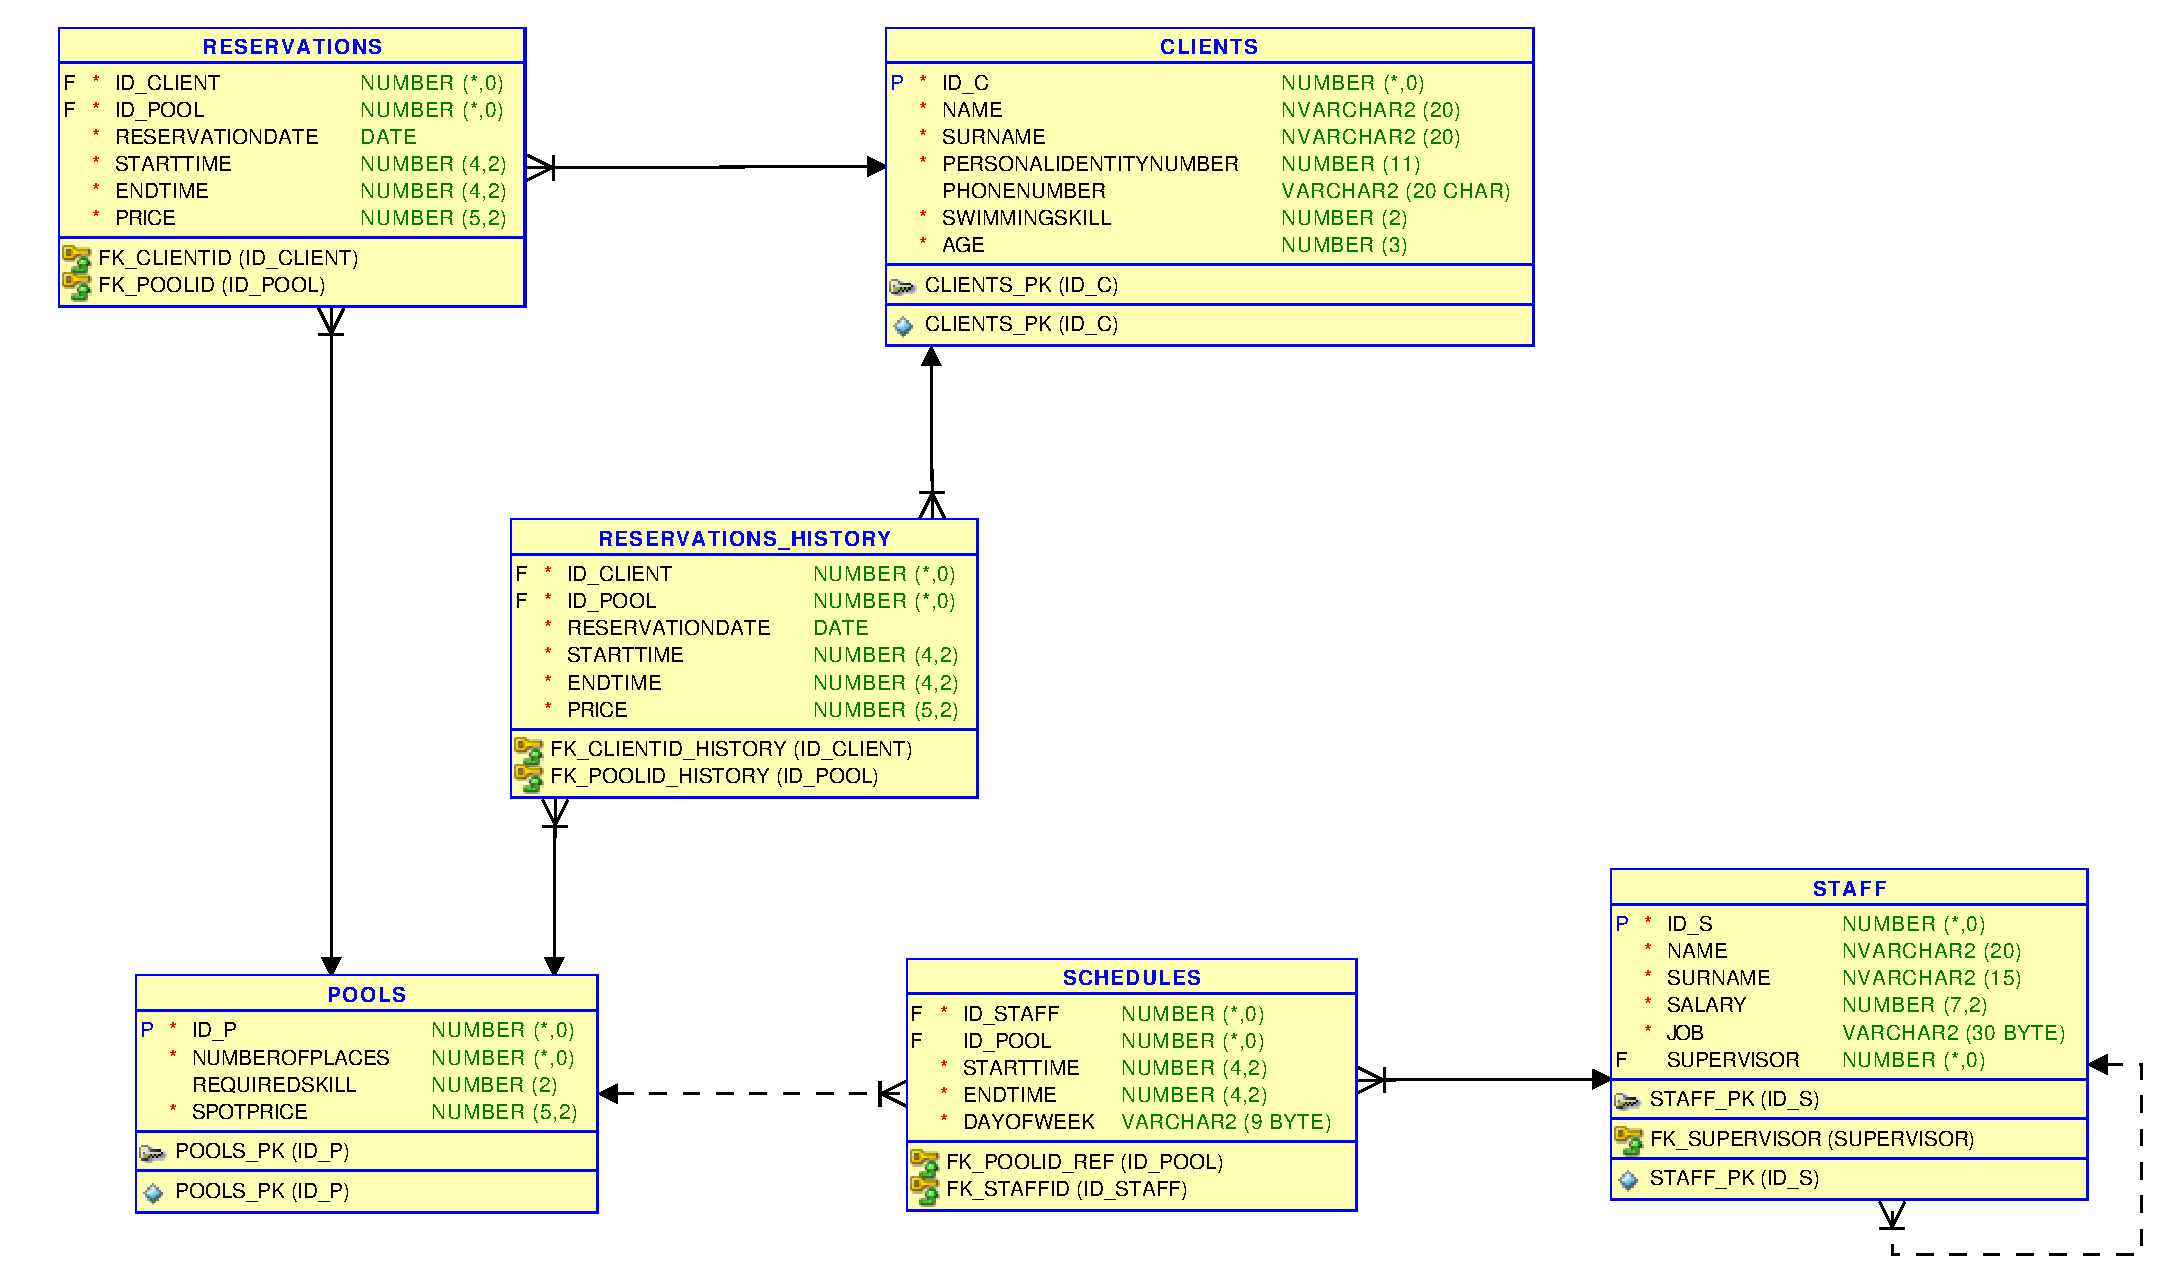
\includepdf[pages=-,pagecommand={\null\vfill\captionof{figure}{Diagram ERD }}]{ERD_DIAGRAM.pdf}

\subsection{Rozwiązanie problemu}

Poniżej zamieszczono dokładny opis implementacji bazy wraz z opisem wykorzystanego systemu zarządzania. W poniższym rozdziale opisano również technologie wykorzystane podczas tworzenia całej bazy danych.

Cały projekt, wraz z dokumentacją, skryptami pozwalającymi na generowanie danych oraz bazy umieszczony został w publicznym repozytorium dostępnym pod poniższym linkiem:
\begin{center}
\textbf{https://github.com/LeszekBlazewski/DataBases1}
\end{center}{}


\subsection{System bazodanowy}

Jako system zarządzania bazą danych wybraliśmy Oracle, ponieważ jest to\textit{ DBMS}, który wykorzystujemy na zajęciach laboratoryjnych i pracowaliśmy już z narzędziami pozwalającymi na łatwą interakcję z podanym systemem.

Poniżej zamieszczono w postaci tabeli dokładne informacje dotyczące wersji wykorzystanej bazy danych i narzędzi pochodnych.

\begin{table}[h!]
\centering
\begin{tabular}{|c|c|}
\hline
\textbf{Narzędzie} & \textbf{Wersja}                                                           \\ \hline
DBMS               & Oracle Database 11g Express Edition Release 11.2.0.2.0 - 64bit Production \\ \hline
PL/SQL             & Release 11.2.0.2.0 - Production                                           \\ \hline
TNS                & TNS for Linux: Version 11.2.0.2.0 - Production                            \\ \hline
NLSRTL             & NLSRTL Version 11.2.0.2.0 - Production                                    \\ \hline
\end{tabular}
\caption{Informacje dotyczące wykorzystanego DBMS}
\label{tab:my-table}
\end{table}


\subsubsection{Wykorzystane technologie}

Ponieważ pracowaliśmy na maszynach z różnymi systemami operacyjnymi - Linux i Windows, zdecydowaliśmy się na konteneryzację bazy danych z użyciem\textit{ Dockera}. Główną zaletą wykorzystanej technologii jest niezależność działania bazy ze względu na środowisko. Kontener pomógł nam w łatwy sposób wystawić bazę na jednym z portów komputera dzięki czemu druga osoba znajdująca się w tej samej sieci \textit{LAN} mogła swobodnie korzystać z bazy i przeprowadzać na niej operacje. Dodatkowym atutem stosowanego rozwiązania jest łatwa skalowalność bazy oraz możliwość łatwej replikacji. Oracle dostarcza możliwość bezpośredniego ściągnięcia obrazu z oficjalnych repozytoriów, a po jego zbudowaniu baza gotowa jest do użytku.

W trakcie implementacji wykorzystaliśmy \textit{Oracle SQL Developer}, jako główne źródło pisania zapytań oraz tworzenia tabel. Niemniej jednak, korzystaliśmy również z narzędzia \textit{SQL PLUS}, które pozwoliło na szybką interakcję z bazą danych z poziomu linii komend/terminala.

Podczas projektowania diagramu \textit{ERD}, również wykorzystaliśmy rozwiązanie oferowane przez Oracle - \textit{SQL Data modeler}, ponieważ dostępne ono było jako dodatek do \textit{SQL Developera} i pozwalało w prosty sposób, wymodelować wybrane encje oraz wiązania między nimi.

Dane umieszczane w bazie wygenerowane zostały przy pomocy skryptów napisanych w języku \textit{Python}, gdzie posłużono się biblioteką \textit{Faker}, która udostępnia funkcje pozwalające na generowanie losowych danych z wielu dziedzin. Dane generowane był w postaci plików w formacie \textit{.csv}, które następnie ładowane były do bazy.

\textit{SQL*Loader}, pozwolił w prosty sposób z poziomu linii komend ładować wcześniej wygenerowane dane, jednocześnie dostarczając informacje o ich poprawności oraz ilości wczytanych rekordów.

Ostatnim z wykorzystanych narzędzi był \textit{Oracle Data Pump}, dostępny od wersji Oracle\linebreak Database 10G. Narzędzie pozwoliło na wygenerowanie pełnego zrzutu bazy, który posłużyć może do wygenerowania identycznej instancji na innym hoście.

\subsubsection{Utworzenie bazy danych}

Najszybszym sposobem wygenerowanie bazy danych jest skorzystanie z narzędzia \textit{Oracle Data Pump}, które pozwala zaimportować cały plik o rozszerzeniu \textit{.dmp}, który wygeneruje poprawnie całą instancję zaimplementowanej bazy danych. Skrypt ten został zamieszczono w repozytorium. Podczas eksportowania danych posłużono się flagą \textit{FULL}, dzięki czemu skrypt wygeneruje identyczną instancję bazy danych wraz z wszystkimi potrzebnymi elementami wymaganymi do poprawnego funkcjonowania.

Poniższy rozdział zawiera zestaw instrukcji pozwalający na wygenerowanie bazy danych, która realizuje wszystkie wymagania zdefiniowane w rozdziale \ref{Wymagania}. Wraz z implementacją w języku \textit{SQL}, zamieszczono również opisy, które ilustrują realizację danych wymagań projektowych.

\subsubsection{Implementacja obiektów}

Pierwszą relację, którą utworzyliśmy na podstawie wcześniej zdefiniowanego diagramu \textit{ERD} była tabela odpowiedzialna za przechowywanie danych klientów. Wraz z utworzeniem tabeli, utworzyliśmy sekwencję, która pozwala na generowanie kolejnych liczb całkowitych o wartościach unikalnych. Sekwencja wywoływana była z Triggera, który automatycznie wstawiał kolejną wartość w kolumnie \textit{ID\_C} w momencie dodawania nowego wiersza. Zgodnie z zdefiniowanymi dziedzinami, na kolumny nałożono również instrukcje \textit{CHECK} sprawdzające poprawność wstawianych wartości.

\begin{minted}{SQL}
CREATE TABLE CLIENTS 
( ID_C NUMBER(*, 0) NOT NULL 
, NAME NVARCHAR2(20) NOT NULL 
, SURNAME NVARCHAR2(20) NOT NULL 
, PERSONALIDENTITYNUMBER NUMBER(11, 0) NOT NULL 
, PHONENUMBER VARCHAR2(20 CHAR) 
, SWIMMINGSKILL NUMBER(2, 0) NOT NULL 
, AGE NUMBER(3, 0) NOT NULL
, CONSTRAINT check_name CHECK (NAME IS NOT NULL) 
, CONSTRAINT CLIENTS_PK PRIMARY KEY 
  ( ID_C )
  USING INDEX 
  ( CREATE UNIQUE INDEX CLIENTS_PK ON CLIENTS (ID_C ASC)) ENABLE
)
\end{minted}

\begin{minted}{SQL}
create or replace TRIGGER CLIENT_INC 
BEFORE INSERT ON CLIENTS
FOR EACH ROW
BEGIN
  SELECT CLIENT_SEQ.NEXTVAL
  INTO   :new.ID_C
  FROM   dual;
END;
\end{minted}

Następnie utworzyliśmy tabelę \textit{POOLS}, która odpowiedzialna była za przechowywanie danych związanych z obecnym stanem basenów. Analogicznie do poprzednich instrukcji, stworzyliśmy sekwencję oraz Trigger odpowiedzialne za generowanie unikalnych wartości dla kolumy \textit{ID\_P}.

\begin{minted}{SQL}
CREATE TABLE POOLS 
(
  ID_P NUMBER(*, 0) 
, NUMBEROFPLACES NUMBER(*, 0) 
, REQUIREDSKILL NUMBER(2, 0) 
, SPOTPRICE NUMBER(5, 2) 
, CONSTRAINT POOLS_PK PRIMARY KEY 
  ( ID_P )
  USING INDEX 
  ( CREATE UNIQUE INDEX POOLS_PK ON POOLS (ID_P ASC) )
  ENABLE 
) 
ALTER TABLE POOLS
ADD CONSTRAINT SYS_C007002 CHECK 
("ID_P" IS NOT NULL)
ENABLE;

ALTER TABLE POOLS
ADD CONSTRAINT SYS_C007003 CHECK 
("NUMBEROFPLACES" IS NOT NULL)
ENABLE;

ALTER TABLE POOLS
ADD CONSTRAINT SYS_C007006 CHECK 
("SPOTPRICE" IS NOT NULL)
ENABLE;

\end{minted}

Wykorzystując dwie poprzednio zaimplementowane relacje, utworzyliśmy tabelę odpowiedzialną za przechowywanie rezerwacji, która odwzorowuje przy pomocy kluczy obcych relację pomiędzy klientami a basenami.
Jednym z wymagań projektowych była możliwość bieżącego monitorowania liczby dostępnych miejsc na basenach oraz cykliczna archiwizacja starszych rezerwacji. W celu spełnienia podanego warunku zdefiniowaliśmy dwie identyczne tabele, gdzie jedna odpowiedzialna była za przechowywanie obecnie trwających rezerwacji, natomiast druga zawiera jedynie dane, które były cyklicznie usuwane. W ten sposób odciążamy relację przechowującą rezerwacje oraz możemy na bieżąco monitorować stan basenów.

Ważny aspekt stanowi również zdefiniowanie operacji \textit{ON DELETE CASCADE}, ponieważ pozwala ona na zachowanie integralności w przypadku usuwania rekordów z tabeli \textit{CLIENTS} lub \textit{POOLS}. W momencie usunięcia rekordu z podanych tabel, automatycznie usuwana jest rezerwacja z tabeli \textit{RESERVATIONS}, która odnosiła się do krotek w podanych tabelach.

Poniżej zamieszczono jedynie definicję jednej z tabel, ponieważ druga wygenerowana została z identycznego skryptu, w którym podmieniono jedynie nazwę tabeli.

\newpage

\begin{minted}{SQL}
CREATE TABLE RESERVATIONS 
(
  ID_CLIENT NUMBER 
, ID_POOL NUMBER(*, 0) 
, RESERVATIONDATE DATE 
, STARTTIME NUMBER(4, 2) 
, ENDTIME NUMBER(4, 2) 
, PRICE NUMBER(5, 2) 
)
ALTER TABLE RESERVATIONS
ADD CONSTRAINT FK_CLIENTID FOREIGN KEY
( ID_CLIENT )
REFERENCES CLIENTS
( ID_C )
ON DELETE CASCADE ENABLE;
ALTER TABLE RESERVATIONS
ADD CONSTRAINT FK_POOLID FOREIGN KEY
( ID_POOL )
REFERENCES POOLS
( ID_P )
ON DELETE CASCADE ENABLE;
ALTER TABLE RESERVATIONS
ADD CONSTRAINT SYS_C007008 CHECK 
("ID_CLIENT" IS NOT NULL)
ENABLE;
ALTER TABLE RESERVATIONS
ADD CONSTRAINT SYS_C007011 CHECK 
("ID_POOL" IS NOT NULL)
ENABLE;
ALTER TABLE RESERVATIONS
ADD CONSTRAINT SYS_C007013 CHECK 
("RESERVATIONDATE" IS NOT NULL)
ENABLE;
ALTER TABLE RESERVATIONS
ADD CONSTRAINT SYS_C007014 CHECK 
("STARTTIME" IS NOT NULL)
ENABLE;
ALTER TABLE RESERVATIONS
ADD CONSTRAINT SYS_C007015 CHECK 
("ENDTIME" IS NOT NULL)
ENABLE;
ALTER TABLE RESERVATIONS
ADD CONSTRAINT SYS_C007016 CHECK 
("PRICE" IS NOT NULL)
ENABLE;

\end{minted}

\newpage

Następnie utworzyliśmy tabelę, która odpowiedzialna jest za przechowywanie danych pracowników. Aby zrealizować wymaganie dotyczące możliwości posiadana nadzorcy przez danego pracownika, posłużyliśmy się relacją zwrotną, zaimplementowaną przy pomocy klucza obcego wskazującego na ta samą tabelę. Ponieważ posiadanie nadzorcy jest opcjonalne, w momencie usunięcia osoby, która była kierownikiem innych pracowników, wszystkie rekordy odnoszące się do danej krotki w kolumnie \textit{SUPERVISOR} wstawianą mają wartość \textit{NULL}.

\begin{minted}{SQL}
CREATE TABLE STAFF 
(
  ID_S NUMBER(*, 0) 
, NAME NVARCHAR2(20) 
, SURNAME NVARCHAR2(15) 
, SALARY NUMBER(7, 2) 
, JOB VARCHAR2(30 BYTE) 
, SUPERVISOR NUMBER 
, CONSTRAINT STAFF_PK PRIMARY KEY 
  ( ID_S )
  USING INDEX 
  ( CREATE UNIQUE INDEX STAFF_PK ON STAFF (ID_S ASC) ) ENABLE 
)
ALTER TABLE STAFF
ADD CONSTRAINT FK_SUPERVISOR FOREIGN KEY
( SUPERVISOR )
REFERENCES STAFF
( ID_S )
ON DELETE SET NULL ENABLE;
ALTER TABLE STAFF
ADD CONSTRAINT SYS_C006996 CHECK 
("ID_S" IS NOT NULL)
ENABLE;
ALTER TABLE STAFF
ADD CONSTRAINT SYS_C006998 CHECK 
("NAME" IS NOT NULL)
ENABLE;
ALTER TABLE STAFF
ADD CONSTRAINT SYS_C006999 CHECK 
("SURNAME" IS NOT NULL)
ENABLE;
ALTER TABLE STAFF
ADD CONSTRAINT SYS_C007000 CHECK 
("SALARY" IS NOT NULL)
ENABLE;
ALTER TABLE STAFF
ADD CONSTRAINT SYS_C007001 CHECK 
("JOB" IS NOT NULL)
ENABLE;

\end{minted}

\newpage

Ostatnią utworzoną relacją była tabela \textit{SCHEDULES}, która odpowiedzialna była za przechowywanie danych dotyczących zmian danych pracowników. Wykorzystując tabelę asocjacyjną, rozwiązaliśmy problem redundancji danych występujących w tabeli \textit{STAFF}, tak jak przedstawiono w procesie normalizacji znajdującym się w rozdziale \ref{Redundancja}. Analogicznie do tabeli \textit{RESERVATIONS}, zastosowaliśmy mechanizm automatycznego usuwania rekordów w momencie usunięcia kluczy głównych do których odnoszą się dane krotki.

\begin{minted}{SQL}
CREATE TABLE SCHEDULES 
(
  ID_STAFF NUMBER(*, 0) 
, ID_POOL NUMBER(*, 0) 
, STARTTIME NUMBER(4, 2) 
, ENDTIME NUMBER(4, 2) 
, DAYOFWEEK VARCHAR2(9 BYTE) 
)
ALTER TABLE SCHEDULES
ADD CONSTRAINT FK_POOLID_REF FOREIGN KEY
( ID_POOL )
REFERENCES POOLS
( ID_P )
ON DELETE CASCADE ENABLE;

ALTER TABLE SCHEDULES
ADD CONSTRAINT FK_STAFFID FOREIGN KEY
( ID_STAFF )
REFERENCES STAFF
( ID_S )
ON DELETE CASCADE ENABLE;

ALTER TABLE SCHEDULES
ADD CONSTRAINT SYS_C007017 CHECK 
("ID_STAFF" IS NOT NULL)
ENABLE;

ALTER TABLE SCHEDULES
ADD CONSTRAINT SYS_C007019 CHECK 
("STARTTIME" IS NOT NULL)
ENABLE;

ALTER TABLE SCHEDULES
ADD CONSTRAINT SYS_C007020 CHECK 
("ENDTIME" IS NOT NULL)
ENABLE;

ALTER TABLE SCHEDULES
ADD CONSTRAINT SYS_C007021 CHECK 
("DAYOFWEEK" IS NOT NULL)
ENABLE;

\end{minted}

\subsubsection{Wprowadzanie danych}

Postanowiliśmy zaimplementować własny generator danych z wykorzystaniem języka Python, ponieważ posiada on bogaty zestaw bibliotek, które znacznie ułatwiają cały proces tworzenia skryptów. Aby przyśpieszyć proces ładowania danych do bazy, dane generowaliśmy do formatu \textit{csv} a następni przy pomocy \textit{SQL*Loadera} wstawialiśmy do bazy.

Dane generowane były przy pomocy biblioteki \textit{Faker}, która pozwala na wyciąganie informacji z wielu dziedzin zależnych od regionu. Dzięki takiemu rozwiązaniu mogliśmy generować poprawne imiona i nazwisko osób z polskimi literami oraz numery pesel. Do konwertowania danych do formatu \textit{csv} posłużyliśmy się biblioteka \textit{Pandas}, która udostępnia gotowy zestaw funkcji, pozwalający na wykonywanie wszystkich operacji związanych z odczytem, zapisem oraz formatowaniem. Do generowania losowych wartości liczbowych wykorzystaliśmy bibliotekę random. Aby wygenerować odpowiednie wartości dla danych wymagających większej precyzji wykorzystaliśmy bibliotekę \textit{numpy}.

W pierwszej kolejności należy wygenerować dane w formacie \textit{.csv} z wykorzystaniem skryptów zamieszczonych w repozytorium. Po sklonowaniu i przejściu do folderu \textit{DataLoaders} należy wykonać poniższą komendę, która wygeneruje pięć plików, które odpowiadają danym w każdej z tabel.

\begin{minted}{python}
python CSVCreator.py
\end{minted}

Poniżej zamieszczono przykładowy skrypt, wykorzystujący bibliotekę \textit{Faker} do generowania danych, które następnie zaimportowane zostaną do tabeli \textit{CLIENTS}. Każdy z skryptów zawiera komentarze pozwalające lepiej zrozumieć zamysł danej implementacji. Pozostałe skrypy dostępne są w repozytorium, do którego link zamieszczono powyżej.

\newpage

\begin{minted}{python}
from random import randint
from DataGenerator import DataGenerator

class ClientDataGenerator(DataGenerator):
    """ Generates data for client table """

    def __init__(self, faker):
        super().__init__(faker)
        self.names = []
        self.surnames = []
        self.social_numbers = []
        self.phone_numbers = []
        self.swimming_skills = []
        self.ages = []

    def generate_table_data(self, number_of_rows):
        for _ in range(0, number_of_rows//4):
            self.names.append(self.fake.first_name())
            self.surnames.append(self.fake.last_name())
            social_number_string = self.create_valid_social_number()
            self.social_numbers.append(social_number_string)
            self.ages.append(self.calculate_age_based_on_social_number(social_number_string))
            self.swimming_skills.append(randint(1, 10))
            shouldGetNumber = randint(1, 5)
            # phone number is optional so leave it blank sometimes
            if shouldGetNumber in (1, 2, 3, 4):
                self.phone_numbers.append(self.fake.phone_number())
            else:
                self.phone_numbers.append('')

        self.table_data = {
            'NAME': self.names,
            'SURNAME': self.surnames,
            'PERSONALITYIDENTITYNUMBER': self.social_numbers,
            'PHONENUMBER': self.phone_numbers,
            'SWIMINGSKILL': self.swimming_skills,
            'AGE': self.ages
        }

    def create_valid_social_number(self):
        """ We don't want to allow clients with ssn starting with 1 because they are to young """

        social_number_string = self.fake.ssn()

        while social_number_string[0] == '1':
            social_number_string = self.fake.ssn()
        else:
            return social_number_string

\end{minted}

Następnie należy utworzyć pliki o rozszerzeniu \textit{.ctl}, które wykorzystywane są przez \textit{SQL*Loadera}, \linebreak do poprawnego zaimportowania danych. Poniżej zamieszczono przykładowy plik o nazwie \linebreak \textit{table\_CLIENTS.ctl} definiujący sposób importowania danych, natomiast reszta udostępniona została w repozytorium.

\begin{minted}{SQL}
load data 
CHARACTERSET UTF8
infile '/databaseData/ClientData.csv' 
append
into table CLIENTS
fields terminated by ','
(ID_C,NAME,SURNAME,PERSONALIDENTITYNUMBER,PHONENUMBER,SWIMMINGSKILL,AGE)
\end{minted}

Ostatnim krokiem, który pozwoli zaimportować dane do bazy danych, jest wykorzystanie narzędzia \textit{SQL*Loader}, korzystając z wcześniej zdefiniowane pliki o rozszerzeniu \textit{.ctl}. Poniżej zamieszczono kolejne komendy wykorzystane do zaimportowania danych do bazy Oracle znajdującej się w kontenerze o nazwie \textit{oracleDb}. Baza zdefiniowana została dla użytkownika \textit{Beard}, dla którego hasło dostępu przyjmowało wartość \textit{Test1}, a \textit{SID} równy był \textit{XE}.

\begin{minted}{bash}
# Polecenia wykonywać należy z folderu /DataBases/dataLoadersCtl
# Przekopiowanie folderu z plikami .ctl do kontenera
docker cp Ctls/. oracleDb:/Ctls
# Przekopiowanie folderu z danymi w plikach csv do kontenera
docker cp databaseData/. oracleDb:/databaseData
# Połączenie się z kontenerem z wykorzystaniem powłoki bash
docker exec -it oracleDb bash
# Przejście do odpowiedniego foldera i nadanie uprawnień do wykonania pliku
cd ./Ctls && chmod +x ./loadData.sh
# Wykorzystanie narzędzia SQL*Loader przy pomocy zdefiniowanego skryptu
./loadData.sh
\end{minted}

Analogicznie do przedstawionego sposobu zaimportowano dane do każdej z tabel, umieszczonych w bazie danych.
Poniżej zamieszczono rezultat importowania danych do tabeli \textit{CLIENTS}, dostarczony przez narzędzie \textit{sqlldr}. Typ danych odczytywany przez narzędzie nie jest zgodny z typami danych kolumn w bazie, lecz podczas wstawiania, dane ulegają konwersji i zostają poprawnie zapisane.

\newpage

\begin{figure}[h!]
\centering
\includegraphics[scale=1.7]{CTL.png}
\caption{Rezultat wykorzystania narzędzia SQL*Loader}
\end{figure}

\newpage

\subsubsection{Przykładowe zapytania w języku SQL, pozwalające realizować typowe operacje}

W poniższym rozdziale zamieszczono przykładowe zapytania, pozwalające na realizację podstawowych procedur takich jak zaprezentowanie danych dotyczących wybranych klientów, udzielenie podwyżki wybranym pracownikom czy usunięcie wybranych rekordów.

DEX DEX DEX DEX DEX DEX DEX DEX DEX DEX DEX DEX 

\subsubsection{Zastosowane restrykcje, triggery, sekwencje, procedury i joby}

Podczas implementacji bazy danych polegaliśmy na rozwiązaniach dostarczonych przez Oracle, które znacznie uprościły realizację wymaganych funkcjonalności. Poniżej zamieszczono zestaw operacji wraz z komentarzami, które wyjaśniają sposób implementacji oraz realizowane zadanie.

\subsubsection{Procedury}

Ponieważ generowaliśmy dane przy pomocy własnych skryptów, podczas pierwszych ładowań danych do bazy, dochodziło do wielu błędów, które naruszały integralność bazy. W celu szybkiego wyczyszczenia danych tabel, posługiwaliśmy się instrukcją \textit{TRUNCATE}. Ponieważ w początkowej fazie nie zdefiniowaliśmy kaskadowego usuwania rekordów w tabelach zawierających klucze obce, napisaliśmy dwa poniższe skrypty, które pozwoliły na aktywację lub wyłączenie wszystkich ograniczeń na danych tabelach.

\begin{minted}{SQL}
create or replace PROCEDURE ENABLE_ALL_CONSTRAINT
IS
BEGIN
-- Enable all constraint except foreign key
for i IN (select table_name, constraint_name
from user_constraints
where status = 'DISABLED'
and constraint_type!='R')
loop
EXECUTE IMMEDIATE 'alter table'||i.table_name||'enable novalidate constraint'||i.constraint_name;
end loop i;

-- Enable foreign key constraint
for i IN (select table_name, constraint_name
from user_constraints
where constraint_type ='R'
and status = 'DISABLED')
loop
EXECUTE IMMEDIATE 'alter table'||i.table_name||' enable novalidate constraint'||i.constraint_name;
end loop i;
END;

\end{minted}

\newpage

\begin{minted}{SQL}
create or replace PROCEDURE DISABLE_ALL_CONSTRAINT
IS
BEGIN
-- Disable foreign key constraint
for i IN (select table_name, constraint_name
from user_constraints
where constraint_type ='R'
and status = 'ENABLED')
loop
EXECUTE IMMEDIATE 'alter table'||i.table_name||' disable constraint'||i.constraint_name;
end loop i;

-- Disable rest of the constraint
for i IN (select table_name, constraint_name
from user_constraints
where status = 'ENABLED')
loop
EXECUTE IMMEDIATE 'alter table'||i.table_name||' disable constraint'||i.constraint_name;
end loop i;
END;

\end{minted}

Ostatnią ze zdefiniowanych procedur była implementacja odpowiedzialna za archiwizację rekordów z tabeli \textit{RESERVATIONS}, których data i czas zakończenia rezerwacji starsze były od obecnej daty i godziny.  Cała procedura realizowała trzy zasadnicze etapy w których skład wchodziły:
\begin{itemize}
    \item Selekcja wszystkich rekordów, które należało zarchiwizować.
    \item Przeniesienie znalezionych rekordów do tabeli \textit{RESERVATIONS\_HISTORY}
    \item Aktualizacja liczby wolnych miejsc na basenach, których dotyczyły archiwizowane rezerwacje.
    \item Usunięcie z tabeli \textit{RESERVATIONS} odpowiednich rekordów.
\end{itemize}

Do uzyskania obecnej daty posłużono się funkcją \textit{CURRENT\_DATE}, natomiast obecną godzinę obliczono na podstawie funkcji \textit{CURRENT\_TIMESTAMP}. Było to koniecznie ponieważ godzina zakończenia rezerwacji przechowywana była jako liczba.

Następnie zdefiniowano własny typ \textit{ GROUPED\_POOLS\_DATA}, który odpowiedzialny był za tymczasowe przechowywanie danych, uzyskanych w wyniku zliczania ilości miejsc, które należy przywrócić dla danego basenu. Dzięki grupowaniu znacznie ograniczamy ilość wykonywanych funkcji \textit{UPDATE}, które aktualizują miejsca dostępne na basenach. W zapytaniu posłużono się instrukcją \textit{BULK COLLECT INTO}, która znacznie przyśpieszyła proces wykonywania całego zapytania. Następnie wykorzystano pętlę \textit{FORALL}, na uzyskanych danych, która również jest bardziej wydajna od pozostałych instrukcji iteracyjnych.

Poniżej zamieszczony został cały skrypt realizujący wszystkie zdefiniowane operacje.

\newpage

\begin{minted}{SQL}
create or replace PROCEDURE ARCHIVE_RESERVATIONS AS
currentDate DATE;
currentTime NUMBER;
-- temporary table for storing grouped result of reservations group by
TYPE GROUPED_POOLS_DATA IS RECORD(
    id_pool NUMBER,  -- Stores rows with poll id
    total_number_of_places NUMBER ); -- and total number of outdate reservations for each pool
-- declare the type of table
TYPE archived_reservations_t IS TABLE OF GROUPED_POOLS_DATA;
-- declare the actual table which will store the result
archived_reservations archived_reservations_t; 
BEGIN
  -- get current date without time
  currentDate := TRUNC(CURRENT_DATE);
  -- get current hour with minutes as number
  currentTime := EXTRACT(HOUR from current_timestamp) + EXTRACT(MINUTE from current_timestamp)/60; 
    
  -- Insert into RESERVATIONS_HISTORY table all reservations which date is older
  -- than current date or equal to it and endtime is older than current time
  INSERT INTO reservations_history
  SELECT * FROM RESERVATIONS
  WHERE reservationdate < currentDate OR (reservationdate=currentDate AND endtime <= currenttime);
  
  -- Calculate for each pool the sum of occupied places by reservations which will be deleted
  SELECT id_pool, COUNT(id_pool) BULK COLLECT INTO archived_reservations
  FROM RESERVATIONS
  WHERE reservationdate < currentDate OR (reservationdate=currentDate AND endtime <= currenttime)
  GROUP BY id_pool;
  
  -- Iterate over each row and update the correct pool
  FORALL pool_index IN 1 .. archived_reservations.COUNT SAVE EXCEPTIONS
    UPDATE POOLS
    SET numberofplaces=numberofplaces + archived_reservations(pool_index).total_number_of_places
    WHERE id_p = archived_reservations(pool_index).id_pool;
    
  -- Delete the rows from RESERVATIONS table
  DELETE FROM RESERVATIONS
  WHERE reservationdate < currentDate OR (reservationdate=currentDate AND endtime <= currenttime);
END ARCHIVE_RESERVATIONS;
\end{minted}


\subsubsection{Joby}

DBMS Oracle, udostępnia przy pomocy Jobów możliwość planowania oraz cyklicznego wykonywania zapisanych procedur. Wykorzystaliśmy tą instrukcję aby zrealizować wymaganie dotyczą automatyzacji archiwizacji przedawnionych rezerwacji. Job ustawiony został w taki sposób aby co pół godziny wykonywał wcześniej zdefiniowaną procedurę. Jako daty początku i końca ustaliliśmy wartość \textit{NULL}, ponieważ chcieliśmy aby zadanie wykonywane było nieustannie, z możliwością zatrzymania go przez użytkownika.

\begin{minted}{SQL}
BEGIN
    DBMS_SCHEDULER.CREATE_JOB (
            job_name => 'ARCHIVE_RESERVATIONS_JOB',
            job_type => 'STORED_PROCEDURE',
            job_action => 'ARCHIVE_RESERVATIONS',
            number_of_arguments => 0,
            start_date => NULL,
            repeat_interval => 'FREQ=MINUTELY;INTERVAL=30',
            end_date => NULL,
            enabled => TRUE,
            auto_drop => FALSE,
            comments => 'Removes old rows from reservation table, inserts them into
            reservations_history and updates number of places for required pools');
END;
\end{minted}

\subsubsection{Triggery}

Kluczową rolę podczas definicji tabel odegrały triggery, które pozwalają na wykonywanie instrukcji krótko przed daną operacją na tabeli oraz po jej wykonaniu. Główną zaletą triggerów jest możliwość interakcji z danymi z innych tabel w momencie wykonywania zapytania na całkowicie innej tabeli. W ten sposób możemy na przykład sprawdzać czy liczba dostępnych miejsc na basenie na który próbujemy dodać rezerwację nie wynosi zero. Triggery pozwalają również na wykorzystanie sekwencji do automatycznego generowania \textit{ID}, dzięki czemu zdejmujemy odpowiedzialność z użytkownika dotyczącą podawania unikalnych wartości dla tej kolumny.

Pierwszy zdefiniowany trigger pozwolił na zachowanie integralności bazy danych dotyczącej ograniczonej liczby miejsc na każdym z basenów oraz możliwości rezerwacji przez klientów jedynie na baseny dla których poziom umiejętności jest mniejszy lub równy poziomowi danego klienta. Cała operacja wykonywana była przed każdym poleceniem \textit{INSERT} do tabeli \textit{RESERVATIONS} i w przypadku nie spełnienia jednego z warunków całość była odrzucana a \textit{DBMS} zgłaszał wyjątek, informując użytkownika o naruszonym warunku.

\newpage

\begin{minted}{SQL}
create or replace TRIGGER "VALID_RESERVATION" BEFORE INSERT OR UPDATE ON RESERVATIONS
FOR EACH ROW
DECLARE
    --declare variables section
    clientSkillLevel number;
    poolSkillLevel number;
    availableSpots number;
    skill_exce EXCEPTION;       --thrown when client does not meet required skill
    spot_exce EXCEPTION;        --thrown when there aren't any spots left
BEGIN
    -- get skill of the client which places reservation
    SELECT SWIMMINGSKILL INTO clientSkillLevel FROM CLIENTS
    WHERE id_c = :NEW.id_client;
    -- get required skill and number of places for pool on which reservation is made
    -- NVL is required because NUMBEROFPLACES can be null (anyone can swim in it)
    SELECT NVL(REQUIREDSKILL, 0), NUMBEROFPLACES INTO poolSkillLevel, availablespots FROM pools
    WHERE id_p = :NEW.id_pool;
    
    IF clientskilllevel < poolskilllevel THEN
        RAISE skill_exce;
    ELSIF availablespots = 0 THEN
        RAISE spot_exce;
    ELSE -- this means that the whole reservation is valid and we have to update the pool value
        UPDATE POOLS
        SET numberofplaces=numberofplaces - 1
        WHERE id_p = :NEW.id_pool;
    END IF;
    EXCEPTION
        WHEN skill_exce THEN
        DBMS_OUTPUT.PUT_LINE('Client does not meet skill requirements for this pool !');
        raise_application_error(-20000, 'Client does not meet skill requirements for this pool !');
        WHEN spot_exce THEN
        DBMS_OUTPUT.PUT_LINE('Pool does not have any available spots at this time !');
        raise_application_error(-20000, 'Pool does not have any available spots at this time !');
END;
\end{minted}

\newpage

Ostatni zdefiniowany trigger pozwolił na automatyczne naliczanie zniżki dla klientów, którzy byli niepełnoletni lub przekroczyli pułap $75$ lat. Dla osób niepełnoletnich cena rezerwacji wynosiła połowę ceny zdefiniowanej dla danego basenu w tabeli \textit{POOLS} natomiast dla osób starszych rabat wynosił $25\%$.

\begin{minted}{SQL}
create or replace TRIGGER "DISCOUNT_RESERVATION" BEFORE INSERT ON RESERVATIONS
FOR EACH ROW
DECLARE
clientAge number(2);
BEGIN
  -- get client age
  SELECT age INTO clientAge
  FROM clients
  WHERE ID_C = :NEW.ID_CLIENT;
  -- check how old given client is and update aprioprate value when condition is met
  IF (clientAge < 18) THEN
    :new.price := :new.price * 0.5;
  ELSIF (clientAge > 75) THEN
    :new.price := :new.price * 0.75;
  END IF;
END;
\end{minted}

\newpage

\subsection{Podsumowanie}

\subsubsection{Założenia projektowe a uzyskany rezultat}

Wszystkie założenia projektowe dotyczące bazy danych zdefiniowane na początku semestru zostały poprawnie zrealizowane. Dodatkowo w trakcie implementacji poszczególnych encji postanowiliśmy rozwinąć operacje realizowane przez nasz system wykorzystując gamę funkcji udostępnianą przez\textit{ DBMS} w tym między innymi triggery, procedury oraz joby. Uzyskanym rezultatem jest w pełni funkcjonalna baza danych, która pozwala na intuicyjne i sprawne zarządzanie mniejszą pływalnią. Dodatkowym atutem bazy jest łatwa skalowalność oraz możliwość rozbudowy danych encji w zależności od potrzeb klienta.

Jedyną częścią zadania, która nie została zrealizowana jest stworzenie aplikacji, która wykorzystywałaby zaprojektowaną bazę danych. Postanowiliśmy skupić się bardziej na samej bazie, jej poprawnym zaprojektowaniu oraz implementacji, ponieważ aplikacja nie była wymagana. Podjęliśmy decyzję o pominięciu aplikacji, a w zamian zaimplementowaliśmy złożone operacje, które wymagały zgłębienia funkcji oferowanych przez ORACLE oraz podstaw języka \textit{PL/SQL}.

\subsubsection{Wnioski}

Projekt dobrze nakreślił złożoność procesu projektowania baz danych. O ile implementacja zależna od wybranego \textit{DBMS}, jest procesem, który przebiega zazwyczaj sprawnie, tak projektowanie oraz dokładne przemyślenie powiązań pomiędzy encjami, jest procesem czasochłonnym. Poprawne wymodelowanie kawałka świata rzeczywistości wymaga przemyślenia i nawet dla tak małych systemów jak system zarządzania pływalnią stanowi kluczowy aspekt, ponieważ definiuje całą strukturę zapytań do bazy. Podczas tworzenia zapytań staraliśmy się wykorzystać wiedzę zdobytą na zajęciach laboratoryjnych. Zaprezentowane zapytania są przykładem operacji, które wywoływane mogły być z poziomu aplikacji.

Projekt pozwolił nam lepiej zapoznać się z bazą ORACLE, jej strukturą oraz funkcjami oferowanymi przez \textit{DBMS}. Wymagania dotyczące automatycznej archiwizacji rezerwacji oraz naliczanie zniżki dla danych klientów pozwoliły nam lepiej zgłębić techniki języka \textit{PL/SQL} oraz wymuszały na nas zastosowanie funkcji takich jak triggery czy procedury.

Ponieważ baza danych utrzymywana była w kontenerze, rozwinęliśmy również umiejętności związane z możliwością zdalnego zarządzania bazą danych z poziomu linii komend oraz poznaliśmy lepiej funkcje dotyczące samego zarządzania bazą danych od strony administracyjnej. Funkcje te odegrały ważną rolę podczas importowania danych z użyciem \textit{SQL*Loadera} oraz podczas eksportowania całej bazy z wykorzystaniem \textit{ORACLE DATA PUMP}.

\newpage

\begin{thebibliography}{9}

\bibitem{Dr.Olga Siedlecka-Lamch}
Materiały dostępne na stronie Doktor Siedleckiej-Lamch
\\\texttt{http://icis.pcz.pl/~olga/dydaktyka.html}

\bibitem{ORACLE} 
Dokumentacja baz danych udostępniona przez ORACLE
\\\texttt{https://docs.oracle.com/en/database/}
 
\end{thebibliography}

\end{document}
